
\section{A rendszer architektúra}
\label{sec:rendterv}

A rendszer több részből áll, melyen két diák is dolgozik, így két dolgozat is készül. Egyrészt a 3D modell, és másrészt az ehhez tartozó UI. Ezeket foglalja össze az \ref{fig:systemArchBig} ábra.
\begin{figure}[H]
	\centering
	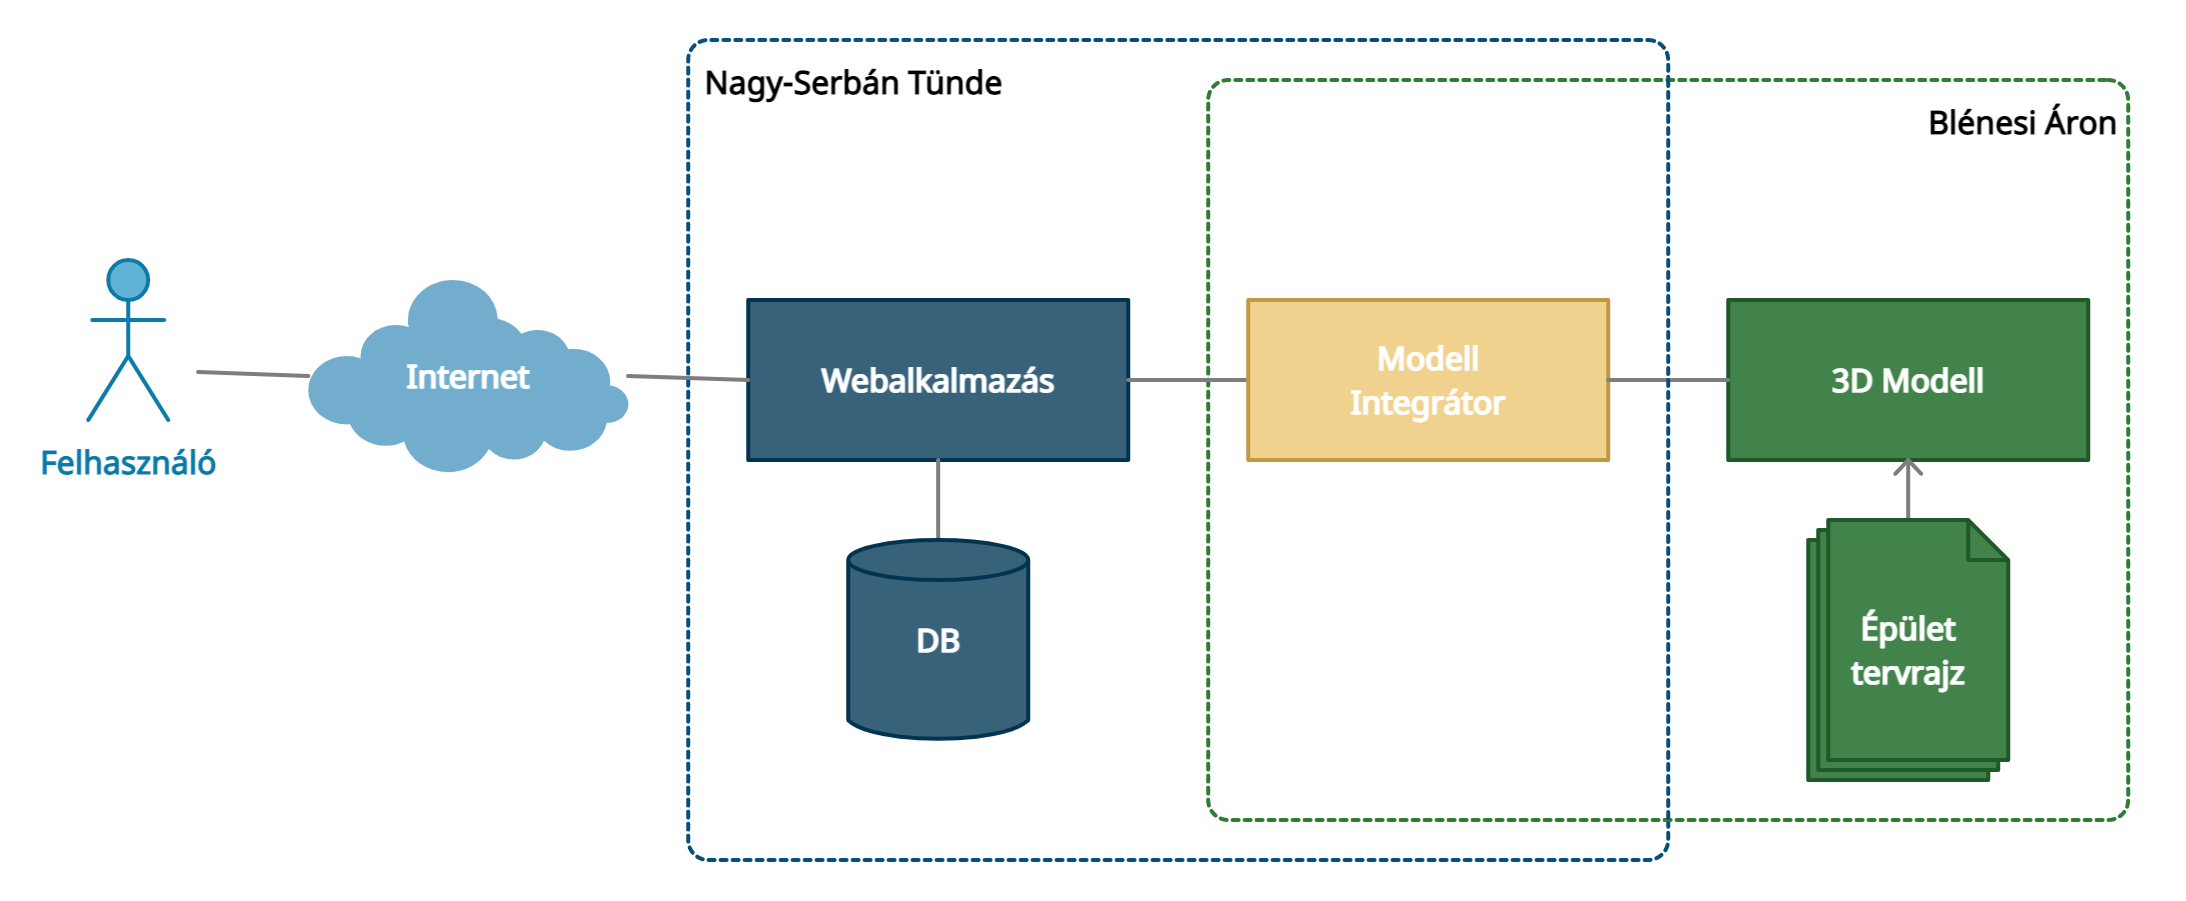
\includegraphics[width=1\linewidth]{figures/images/kozosfazis.png}
	\caption[A teljes rendszer architektúrája]{\textit{A teljes rendszer architektúrája}}
	\label{fig:systemArchBig}
\end{figure}

A 3D modell tervezését, implementálását a kollégám, Blénesi Áron készíti el míg a webalkalmazást, adatbázis tervezést én. A két projektet egy komponensen keresztül kötjük össze. Ez a komponens a web alkalmazáson belül van létrehozva, és általa jelenítődik meg a 3D modell.

A kolléga dolgozata arról szól, hogy a modell hogyan lett megtervezve, elkészítve és nem utolsó sorban hogyan lett beépítve egy weboldalba. A modell az egyetem valós tervrajzai alapján készült el törekedve a pontosságra, hiszen biztosítani szerettük volna a felhasználónak azt az élményt, hogy életnagyságban járhassa be a digitalizált épületet. A feldolgozáshoz használt segédeszköz a Blender, ingyenes modellező software volt. A komplex modell elkészítése után ez exportálásra kerül egy glTF (Grafikus nyelvátviteli formátum) kiterjesztésű fájlba. Ez a fájl majd beépítésre kerül a webalkalmazásba a modell komponensen keresztül. Ez a komponens felel a 3D-s modell megjelenítéséért és az épület bejárási logikájának mevalósításáért. Ezen az oldalon a felhasználó interakcióba léphet a modellel, szabadon bejárhatja azt, illetve úticélt választhat a megadott listából és a kamera egy jólmeghatározott útvonalat követve lépésenként elér a kiválasztott úticélig.
